\documentclass[a4paper,11pt]{article}
\usepackage{latexsym}
\usepackage[polish]{babel}
\usepackage[utf8]{inputenc} 
\usepackage[MeX]{polski}
\usepackage{nicefrac}
\usepackage{listings}
\usepackage{multirow}
\usepackage[normalem]{ulem}
\useunder{\uline}{\ul}{}
\usepackage{float}
%\usepackage[margin=0.6in]{geometry}
\usepackage{graphicx}
\usepackage{multicol}
\lstset{showstringspaces=false}

\author{Marcin Mrugas 122580 \\
		Marcin Drzewiecki 122472}

\title{Przetwarzanie i rozpoznawanie obrazów\\ 
\large{{\bf Sprawozdanie} \\ Projekt 2 -- deskryptor obrazu}} 

\date{20 maja 2018}

\begin{document}

\maketitle 

\section{Metody wyznaczania deskryptora obrazu}

Jeśli nie wskazano inaczej, jako otoczenie punktu należy rozumieć koło o promieniu $ r = 32 $ o środku w danym punkcie.
Przed zastosowaniem metod, na otoczeniu była stosowana normalizacja jasności obrazu, tj. zmiana jasności piksela wg wzoru:

$$ \frac{v_i - min(v)}{max(v)-min(v)},$$
gdzie $v$ -- otoczenie punktu, $v_i$ -- $i$-ty piksel otoczenia.

\subsection{Średnia jasność otoczenia}

\subsubsection{Ekstrakcja}
Najprostsza metoda polegała na wyznaczeniu średniej jasności pikseli w otoczeniu danego punktu.

\subsubsection{Porównanie}
Porównanie deskryptorów polegało badaniu zależności między wyznaczonymi średnimi zgodnie z wzorem:

$$ min(1, \frac{|des_1 - des_2|}{64}) $$

\subsection{Wynik działania}

\begin{figure}[H]
\begin{center}
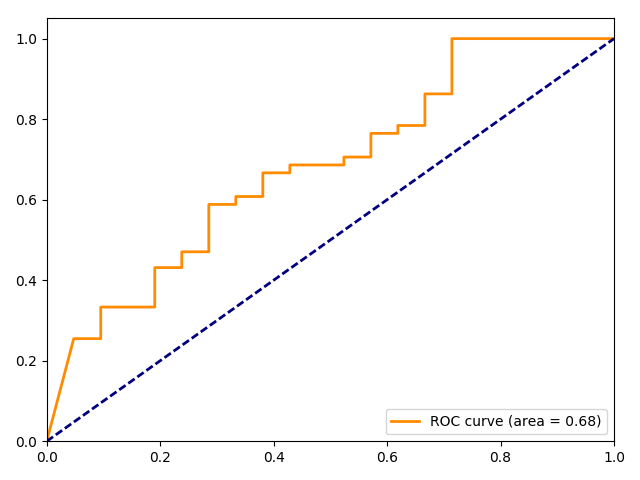
\includegraphics[width=0.7\textwidth]{./img/average.png}
\end{center}
\caption{Wynik działania deskryptora, AUC.}
\end{figure}


\subsection{Momenty Hu}

\subsubsection{Ekstrakcja}
Metoda polegała na wyznaczeniu momentów Hu z otoczenia punktu. 

\subsubsection{Porównanie}
Najpierw wyznaczono dla każdego momentu wartości:
$$ v_i = -sgn(h_i) * log_{10}|h_i|, $$
gdzie $h_i$ oznacza $i$-ty moment Hu, a $sgn(x)$ -- znak liczby $x$.
Następnie porównano dwa wektory $v$ oraz $w$zgodnie ze wzorem:

$$ \sum_{i=1}^{7}|v_i - w_i|$$

\subsection{Wynik działania}

\begin{figure}[H]
\begin{center}
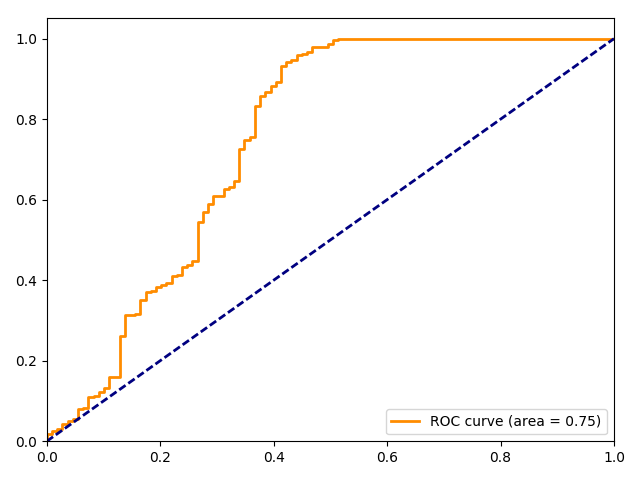
\includegraphics[width=0.7\textwidth]{./img/hu.png}
\end{center}
\caption{Wynik działania deskryptora, AUC.}
\end{figure}

\subsection{Średnie jasności na okręgach}

\subsubsection{Ekstrakcja}
Metoda polegała na wyznaczeniu średniej jasności pikseli oddalonych o $r = 0,1,...,32$ od badanego punktu. 
W ten sposób otrzymano wektor o długości $33$.

\subsubsection{Porównanie}
Dla każdego z współczynników: $a = 0.7, 0.8, 0.9, 1, \frac{1}{0.7}, \frac{1}{0.8}, \frac{1}{0.9}$, wykonywano następujące czynności.
Porównywano pierwsze $\left \lfloor  a \cdot 33 \right \rfloor$ elementów pierwszego wektora oraz tyle samo elementów drugiego wektora. Aby uzyskać odpowiednią długość drugiego wektora dokonywano operacji analogicznej do decymacji w cyfrowym przetwarzaniu sygnałów.
Dzięki temu deskryptor był odporny na skalowanie.
Porównanie dwóch wektorów polegało na wyznaczeniu korelacji ($c_i$) między dwoma wektorami oraz wybranie maksymalnej z wyznaczonych wartości i odjęcie jej od $1$:

$$ 1-max(c) $$

\subsection{Wynik działania}

\begin{figure}[H]
\begin{center}
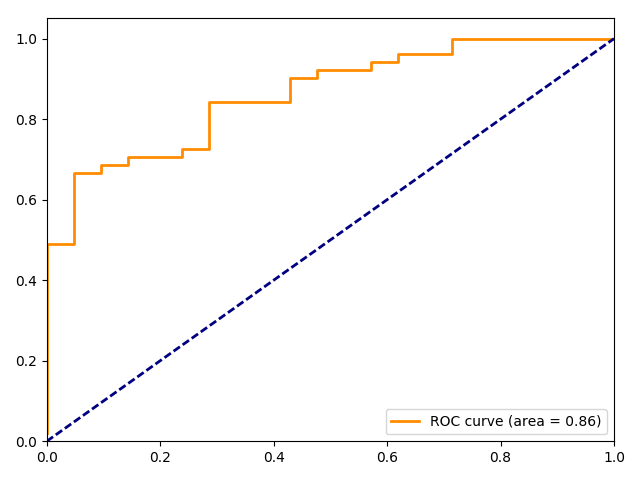
\includegraphics[width=0.7\textwidth]{./img/circle_hist.png}
\end{center}
\caption{Wynik działania deskryptora, AUC.}
\end{figure}

\subsection{Maksymalne jasności na okręgach}

\subsubsection{Ekstrakcja}
Metoda polegała na wyznaczeniu piksela o maksymalnej jasności oddalonego kolejno o $r = 0,1,...,32$ od badanego punktu.
Dla każdego wyznaczonego piksela wyznaczano kąt, jaki tworzy odcinek łączący najjaśniejszy piksel z badanym punktem i prosta równoległa do krawędzi obrazu. 
W ten sposób otrzymano wektor o długości $33$.

\subsubsection{Porównanie}
Dla każdego z współczynników: $\alpha = 0, \frac{\pi}{36}, \frac{2\pi}{36},...\frac{17\pi}{36}$, zwiększano każdą z wartości pierwszego wektora o $\alpha$ oraz porównywano otrzymane wektory w taki sam sposób jak w poprzedniej metodzie, z tą różnicą, że jako ostateczną wartość brano maksymalną wartość bezwzględną z korelacji między wektorami.


\subsection{Wynik działania}

\begin{figure}[H]
\begin{center}
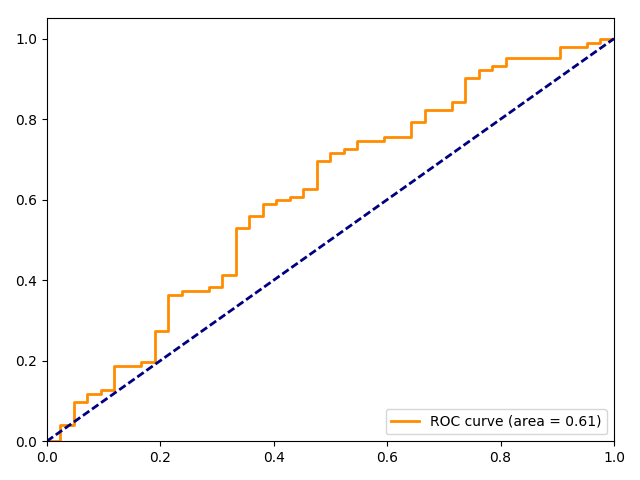
\includegraphics[width=0.7\textwidth]{./img/max_on_circle.png}
\end{center}
\caption{Wynik działania deskryptora, AUC.}
\end{figure}


\subsection{Porównanie jasnoilościowych punktów}

\section{Ekstrakcja}
Metoda opiera się na algorytmie BRIEF z modyfikacjami.
Na początku są losowane punkty należące do okręgu o wielkości rozważanego deskryptora z jednostajnym prawdopodobieństwem. Dla obrazu dla którego jest obliczany deskryptor jest  %TODO
Następnie dla każdego obrazu są porównywane punkty a dokładniej ich jasności które są zapisywane w zależności który punkt z pary był jaśniejszy. Tak stworzony deskryptor to łańcuch zer i jedynek pozwalający na przedstawienie opisu zdjęcia. 

\subsection{Porównanie}
Porównywanie obrazów odbywa się przy pomocy odległości Hamminga.


\subsection{Wynik działania}

\begin{figure}[H]
\begin{center}
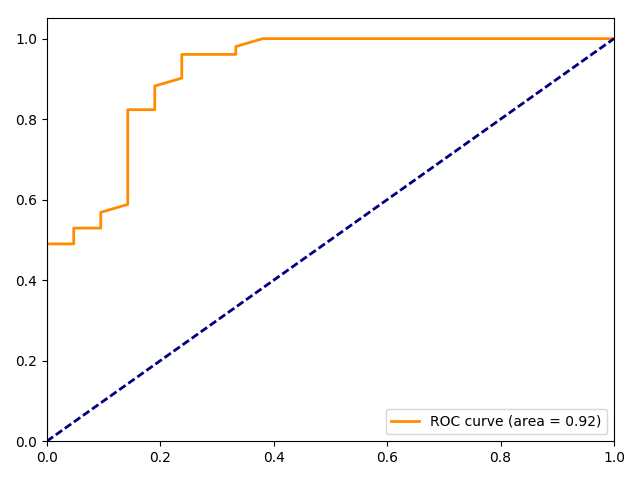
\includegraphics[width=0.7\textwidth]{./img/brief.png}
\end{center}
\caption{Wynik działania deskryptora, AUC.}
\end{figure}

\section{Testowanie}
Aby móc dobrze ocenić działanie deskryptora zostały napisane dwa skrypty umożliwiające sprawdzenie jakości naszego rozwiązania. Pierwszy używa prawdziwych zdjęć z podanego zbioru losując punkty i zapisując ich współrzędne wraz z odpowiadającymi im punktami w odpowiadających zdjęciach. Drugi zaś wybiera losowy fragment i poddaje go transformacją:
\begin{enumerate}
\item rozmycia,
\item korekcji gamma,
\item obrotowi,
\item powiększeniu,
\item kompresji jpg.
\end{enumerate}
\section{Odporność}
\subsection{Rotacja}
<class 'list'>: [0.0, 6.771087646484375e-05, 8.392333984375e-05, 9.72747802734375e-05, 0.00015544891357421875, 0.0001735687255859375, 0.00015354156494140625, 0.00014781951904296875, 0.00018978118896484375, 0.00022983551025390625]

\end{document}  
